%!TEX root = ../main.tex
\part{Calorimetry for Future Colliders}

\chapter{Future $e^+e^-$ linear collider experiments}
\label{chap:FutureColliders}

The Standard Model has been so far a very successful theory in describing physics phenomena up to TeV-scale energies. However, there are still open-questions that the Standard Model fails to answer as discussed in chapter \ref{chap:Theory}.

Currently, the only high energy hadron collider in operation to push the energy frontier is the \textit{Large Hadron Collider} (LHC) at CERN between Switzerland and France. The LHC uses the Large Electron-Positron Collider (\acrshort{lep}) long underground tunnel of 27 km circumference and it is colliding protons at a center-of-mass energy up to $\sqrt{s} = 14$ TeV using superconducting magnets. The LHC is probing the Standard Model to an unprecedented energy scale and searches for new particles beyond the Standard Model. The discovery of the Higgs Boson in 2012 \cite{Aad:2012tfa, Chatrchyan:2012xdj} was one of the major milestones of the LHC. The colliding particles are protons that are composite particles. The collision happens at parton level, carrying a fraction of the proton energy of which the energy is not accessible by the experiment. These collisions are very complex and the initial conditions of the collisions are not known and thus, limits the precision of the measurements. On the other hand, lepton colliders provide a clean environment and a known initial state for precision physics.

A limitation of $e^+e^-$ ring colliders is the maximum achievable collision energy which is limited by the energy losses of the particles due to the synchrotron radiation. Due to the energy and mass dependence of the radiation losses ($\sim E^4/m^4$), a trade-off is needed between the radius of the collider and the maximal energy provided to the machine. In order to minimize the power losses by colliding leptons, it is most likely that the next $e^+e^-$ collider will be a linear accelerator to achieve energies near the TeV scale.

There are currently several proposals for future lepton colliders such as the \textit{Compact Linear Collider} (\acrshort{clic}) \cite{CLIC_CDR}, the Future Circular Collider (\acrshort{fcc}) \cite{Benedikt:2015kqj}, the Circular Electron Positron Collider (\acrshort{cepc}) \cite{CEPC-SPPCStudyGroup:2015csa, CEPC-SPPCStudyGroup:2015esa} and the \textit{International Linear Collider} (\acrshort{ilc}) \cite{ILC_TDR_Vol1}. The most mature project is the ILC which is a polarized lepton collider with a center of mass energy between 250 and 500 GeV upgradable to 1 TeV.

In this chapter, the scientific case for a lepton collider is made in section \ref{sec:ILC_Physics}. Then a short summary of the ILC machine is given in section \ref{sec:ILC}. The two detectors are foreseen to be installed at the ILC interaction point, namely the International Large Detector (\acrshort{ild}) and the Silicon Detector (\acrshort{sid}) are described in section \ref{sec:ILD}. All the information provided in this chapter are based on the ILC Technical Design Report (TDR) \cite{ILC_TDR_Vol1, ILC_TDR_Vol2, ILC_TDR_Vol3.1, ILC_TDR_Vol3.2, ILC_TDR_Vol4} if not stated otherwise.

\section{The case for a lepton collider}
\label{sec:ILC_Physics}

The ILC physics program is complementary to studies done at the LHC. The recent discovery of the Higgs Boson in the 125 GeV range at the LHC, which was for several decades the missing piece of the Standard Model, can be studied with higher precision with the ILC. The probing of the characteristics of the Higgs Boson to a percent level is necessary to validate the current SM and as well in order to be able to observe any deviations to the SM predictions that would be a strong hint for physics beyond the SM. Besides, the ILC would provide many opportunities for the study of new physics, the Z and W Bosons and the top quark. This section will describe few key points of the ILC physics program.

\subsection{Higgs Physics}

The ILC experiment would provide a precise measurement of the Higgs Boson characteristics such as its mass, its full decay width and its coupling to SM particles. At hadron colliders such as the LHC, the Higgs total cross-section is measured under some assumptions. Therefore the measurements of the Higgs properties are model-dependent. The precision on some of the Higgs properties at the LHC is significantly worse than for the ILC \cite{Fujii:2015jha}.

\subsubsection{Higgs mass, Branching Ratio and coupling measurements}

There are two main production modes of the Higgs at the ILC, the \textit{Higgsstrahlung} and \textit{Vector Boson Fusion} (\acrshort{vbf}). The \textit{Higgsstrahlung} process is the production of a Higgs Boson in association with a Z Boson. For the VBF mode, either two Z or W Bosons fuse in a Higgs Boson in association with either an electron-positron pair or neutrino-antineutrino pair. The Feymann diagrams of these processes are shown in figure \ref{fig:HiggsProd}.

\begin{figure}[htbp!]
  \centering
  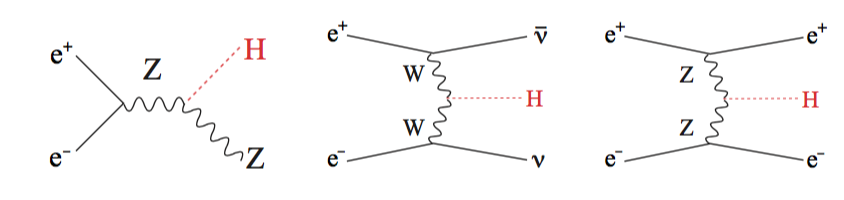
\includegraphics[width=1\linewidth]{chap2/fig/HiggsProd.png}
  \caption{Feymann diagrams for the Higgs production at the ILC at tree level. \cite{ILC_TDR_Vol2}} \label{fig:HiggsProd}
\end{figure}

At $\sqrt{s}$ = 250 GeV, the production cross-section is dominant \cite{Moortgat-Picka:2015yla}. At higher energies around $\sqrt{s}$ = 450 GeV, the VBF production cross-section starts to dominate. The decay modes of the Higgs and their branching ratio are shown in table \ref{table:BRHiggs}. Massless final states decays are possible through heavy loops (top, WW or ZZ loops).

\begin{table}
  \centering
  \caption{Decay modes of the Higgs boson and the branching ratio for a SM Higgs boson at $m_H$ = 125 GeV \cite{}. Others represents $\mu\mu$, $\gamma\gamma$, $Z\gamma$ and invisible.}
  \label{table:BRHiggs}
  \begin{tabular}{@{}ll@{}} \toprule
    Decay Mode & Branching Ratio \\ \midrule
    $H \rightarrow b\bar{b}$ & 57.7\% \\
    $H \rightarrow WW^*$ & 21.5\% \\
    $H \rightarrow ZZ^*$ & 2.6\% \\
    $H \rightarrow gg$ & 8.6\% \\
    $H \rightarrow \tau^+\tau^-$ & 6.3\% \\
    $H \rightarrow c\bar{c}$ & 2.9\% \\
    $H \rightarrow \text{others}$ & < 1\% \\
    \bottomrule
  \end{tabular}
\end{table}

At the ILC, the initial state of the collision is precisely known, offering a unique method to measure the Higgs mass. The \textit{recoil mass measurement}, in the Higgsstrahlung process, aims at reconstructing the Z boson recoiling against the Higgs without the need to reconstruct the Higgs itself, no assumption is made on the decay mode. This enables a model-independent measurement of the Higgs mass, the Higgs couplings and the Higgs full decay width with an unprecedented precision.

Events where the Z decays to a pair of charged leptons ($e^+e^-$ or $\mu^+ \mu^-$) are used due to the excellent tracker resolution of the ILC detectors. The recoil mass $m_{recoil}$ can be calculated as \cite{Yan:2016xyx}
\begin{equation}
  m_{recoil}^2 = (\sqrt{s} - (E_{l^+} + E_{l^-}))^2 -  |\textbf{p}_{l^+} + \textbf{p}_{l^-}|^2
\end{equation}
where $E_{l^j}$ and $\textbf{p}_{l^j}$ are the energy and momentum of the lepton pair from the Z decay. These events can be selected by constraining the invariant mass of the lepton pair to be consistent with the Z mass. A reconstructed recoil mass distribution for $Zh \rightarrow \mu^+\mu^-X$ is shown in figure \ref{fig:HiggsRecoilMuMu}. Combining the results of the $\mu^+\mu^-$ and $e^+e^-$ channels, a statistical precision of 32 MeV on the Higgs mass can be achieved, resulting in an uncertainty of 2.5\% on the production cross-section measurement.

\begin{figure}[htbp]
  \centering
  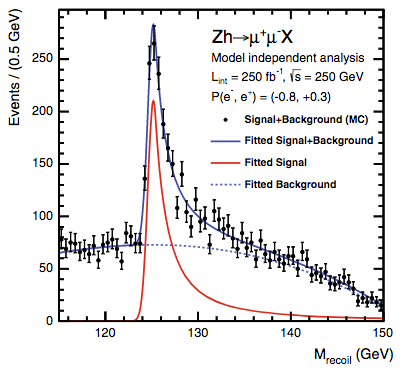
\includegraphics[width=0.5\linewidth]{chap2/fig/HiggsRecoilMuMu.png}
  \caption{The recoil mass distribution for $Zh \rightarrow \mu^+\mu^-X$ at $\sqrt{s}$ = 250 GeV for 250 fb$^{-1}$ integrated luminosity and beam polarisation of (+80\%, -30\%). Simulated with $m_h$ = 125 GeV. \cite{Thomson2016}} \label{fig:HiggsRecoilMuMu}
\end{figure}

At the ILC, the full Higgsstrahlung inclusive production cross-section is proportional to the square of the coupling between the Z and Higgs, $g_{hZZ}$
\begin{equation}
  \sigma(e+e- \rightarrow Zh) \propto g^2_{hZZ}
\end{equation}
The branching ratio of a decay channel is expressed as
\begin{equation}
  BR(h \rightarrow XX) = \frac{\Gamma(h \rightarrow XX)}{\Gamma_{h}}
\end{equation}
where $\Gamma_{h}$ is the full decay width of the Higgs and $\Gamma(h \rightarrow XX)$ is the partial decay width with $\Gamma(h \rightarrow XX) \propto g^2_{hXX}$.

Typically in a collider, the quantity measured is the event rate of a final state corresponding to the product of the production cross-section and BR. Thus the final state cross-section at the ILC for the Higgsstrahlung and VBF production is expressed as
\begin{equation}
  \begin{aligned}
    &\sigma(e^+e^- \rightarrow Zh) \times BR(h \rightarrow XX) \propto \frac{g^2_{hZZ} \cdot g^2_{hXX}}{\Gamma_{h}}\\
    &\sigma(e^+e^- \rightarrow h\nu_e\nu_e) \times BR(h \rightarrow XX) \propto \frac{g^2_{hWW} \cdot g^2_{hXX}}{\Gamma_{h}}
  \end{aligned}
\end{equation}
By measuring the inclusive cross-section $\sigma(e^+e^- \rightarrow Zh)$ with the recoil technique, a direct measure of $g_{hZZ}$ is done. A precision of 1.3\% can be achieved for this coupling for 250 fb$^{-1}$ integrated luminosity. The coupling $g_{hWW}$ for the same final state of the Higgs (e.g. $h \rightarrow bb$) can be expressed as:
\begin{equation}
  g^2_{hWW} \propto g^2_{hZZ} \times \frac{\sigma(e^+e^- \rightarrow h\nu_e\nu_e)}{\sigma(e^+e^- \rightarrow Zh)}
\end{equation}

Therefore, it is only needed to measure the branching ratio $BR(h \rightarrow WW^*)$ to determine $\Gamma_{h}$ via $\sigma(e^+e^- \rightarrow h\nu_e\nu_e) \times BR(h \rightarrow WW^*) \propto \frac{g^4_{hWW}}{\Gamma_{h}}$. All inclusive cross-section measurements can be included into a global fit to minimize the uncertainty on $\Gamma_{h}$. Figure \ref{fig:HiggsCouplings} shows the relative precision achievable for the ILC compared to the LHC. For most of the measurements, the ILC is one order of magnitude more precise than at the LHC and below the percent level precision.

\begin{figure}[htbp]
  \centering
  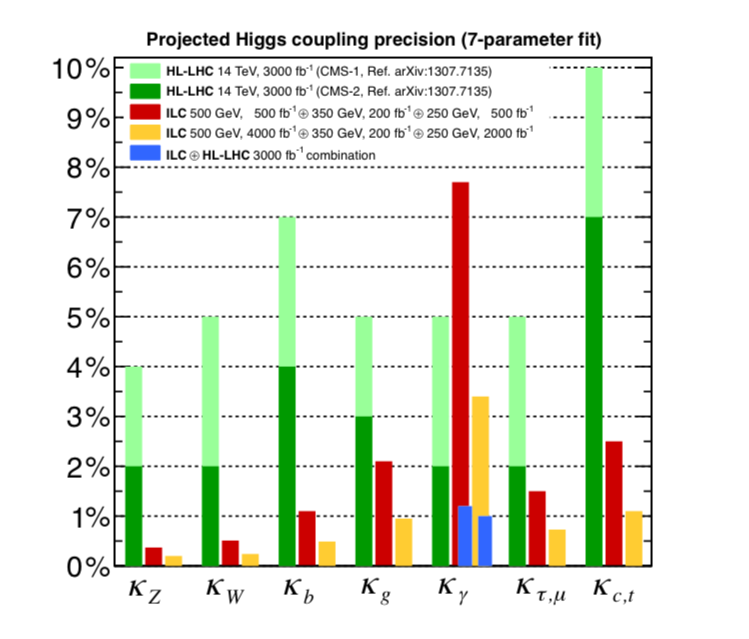
\includegraphics[width=0.7\linewidth]{chap2/fig/HiggsCouplings_LHCComp.png}
  \caption{Relative precision of the Higgs couplings extracted for the ILC in a model-dependent analysis. Projections of the achievable precision on the Higgs couplings for the HL-LHC are shown as well in a pessimistic (CMS-1) and optimistic (CMS-2) case on the systematic uncertainties \cite{Fujii:2015jha}.}  \label{fig:HiggsCouplings}
\end{figure}

There are different models for physics beyond the Standard Model. These models result in deviations, scaling as $1/\Lambda^2_{NP}$, to the predicted Higgs couplings from the SM generally around few percent level \cite{Gupta:2012mi}. For example, in a composite Higgs model, a decrease in all the Higgs couplings is expected. Therefore, searching for deviations in the Higgs couplings measurement gives a way to know if the discovered Higgs is from the Standard Model, a composite particle or whether there is more than one Higgs boson.

\subsubsection{Higgs self-coupling}

The trilinear Higgs self-coupling $\lambda$ determines the shape of the Higgs potential as discussed in chapter \ref{chap:Theory}. It gives an understanding of the nature of the transition from a symmetric state to a broken symmetry state in the electroweak sector \cite{Kajantie:1996mn}. It would give hints about the possibility of CP violation in the Higgs sector and thus information about the origin of baryon-antibaryon asymmetry.

The trilinear coupling can be studied at the ILC via the Higgsstrahlung or VBF production starting at around $\sqrt{s}$ = 350 GeV. The cross-section maximizes at around $\sqrt{s}$ = 600 GeV dominated by the Higgsstrahlung process. Extensive studies \cite{Duerig:2016dvi, Tian:2013qmi} have found that at 500 GeV with 4 ab$^{-1}$ of integrated luminosity combining $H \rightarrow bbbb$ and $H \rightarrow bbWW^*$ channels, a precision of 27\% on the Higgs self-coupling can be achieved. At 1 TeV with 8 ab$^{-1}$ and by combining with the 500 GeV measurement, a precision of around 10\% can be achieved on the trilinear Higgs self-coupling.

\subsection{Electroweak sector}

The ILC gives access to an unprecedented level of precision for the measurement of W and Z masses, widths and couplings. The production processes $e^+e^- \rightarrow W^+W^-$, $e^+e^- \rightarrow ZZ$, $\gamma\gamma \rightarrow W^+W^-$ and triple boson production $e^+e^- \rightarrow VVV$ can be studied.

Currently, the LHC does not constrain much new physics in the electroweak sector and its reach is limited \cite{Alboteanu:2008my}. Therefore with the ILC, vector boson scattering can be studied at the TeV scale to constrain furthermore the Electroweak (EW) sector and search for deviations in the structure of the EW sector of the SM. Many new physics models beyond the SM predict new couplings to the W and Z bosons, thus mixing effects of the new bosons could be detected by the ILC precision measurements.

\subsection{Top mass measurement}

The top quark is the heaviest particle in the Standard Model with a mass of 173.34 $\pm$ 0.27 (stat) $\pm$ 0.71 (syst) GeV \cite{ATLAS:2014wva}. The top quark was discovered at the Tevatron by the CDF and D\O{} experiments \cite{Abe:1995hr, D0:1995jca}, and has only been studied by hadron colliders so far. The ILC would be the first machine to study the top quark using a leptonic initial state.

It is the most strongly coupled particle to the Higgs as the coupling is proportional to the mass (see chapter \ref{chap:Theory}). Many parameters of the Standard Model such as the W, Z couplings and Higgs mass are affected by the top mass via radiative corrections. The top quark is therefore expected to be one of the most promising windows to new physics beyond the Standard Model at the TeV energy scale.

The top quark has a very short lifetime ($10^{-25}$ s), and it decays before hadronization thus the top is a "bare" quark. It decays almost exclusively to $t \rightarrow W^+b$ with the b quark being almost only left-handed polarized. At the ILC, the top quark mass can be measured at the threshold of $\sqrt{s} \sim 2 m_t$ as the machine can be tuned in energy. Thus the shape of the top cross-section production can be measured allowing precise measurement of the top mass $m_t$, width $\Gamma_t$ and strong coupling constant $\alpha_s$. Additionally, the initial beam polarization state can be tuned to enhance the cross-section.

Via this method, the top mass is expected to be measured at the ILC with a statistical precision of around 30 MeV but the final mass is mostly dominated by theoretical uncertainties of around 100-200 MeV.

\subsection{Beyond the Standard Model}

One of the central pillar for a lepton collider is the search for new physics beyond the Standard Model. For direct searches, dark matter is of the main interest such as mono-photon searches similar to mono-jet searches at the LHC \cite{Gustavino:2017dub}. The ILC is complementary to the LHC in covering the phase space of dark matter mass, in the sense that the LHC covers high masses while the ILC covers low couplings and high mediator masses \cite{Habermehl:2017dxh}.

In addition, some regions are not accessible or can be very challenging at the LHC in the case of a degenerate lightest supersymmetric particle (LSP) and the next lightest supersymmetric particle (NLSP) \cite{Baer:2011ec}. The ILC could resolve such degenerate spectrum thus allowing the measurement of SUSY parameters in the order of 5\% \cite{Reuter:2016olv}.

\section{The International Linear Collider (ILC)}
\label{sec:ILC}

The design of the International Linear Collider (ILC) has been ongoing for several decades of research and development for linear colliders. The ILC community regroups more than 300 laboratories, institutes and universities worldwide. In this section, a general overview of the ILC machine is given.

\subsection{General Overview}

The ILC is planned to be a 31 km long $e^+e^-$ linear collider to be built in Japan with a baseline design peak luminosity of around $2 \times 10^{34} cm^{-2}s^{-1}$ and a center-of-mass energy of 500 GeV. An upgrade up to 1 TeV center-of-mass energy and a higher luminosity is possible. However, a staging scenario approach starting at 250 GeV is proposed in \cite{Fujii:2017vwa}. It uses superconducting radio-frequency (SCRF) cavities to accelerate electrons and positrons. The project is currently under discussion between the governments and a decision by the end of 2018 should be reached. A schematic of the ILC layout is shown in figure \ref{fig:ILC_schematic}.

\begin{figure}[htbp!]
  \centering
  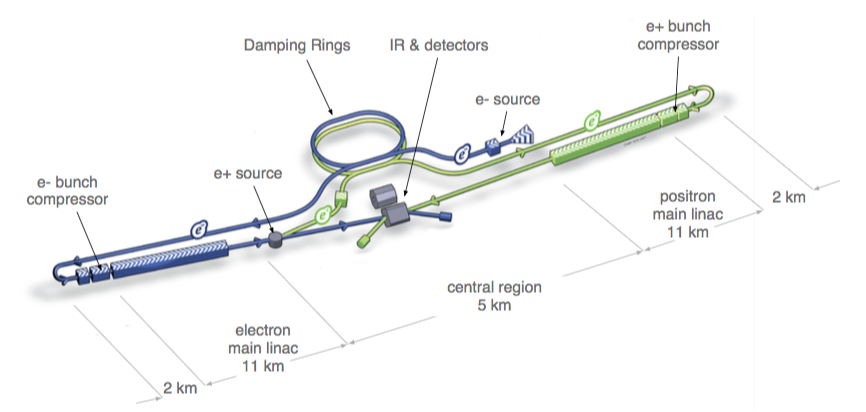
\includegraphics[width=0.8\linewidth]{chap2/fig/ILC_schematic.png}
  \caption{Schematic of the International Linear Collider (not to scale). \cite{ILC_TDR_Vol1}.} \label{fig:ILC_schematic}
\end{figure}

One of the advantages of the ILC is the polarization of beam particles. A polarization up to 80\% for electrons and 30\% for positrons can be achieved. The use of opposite sign polarity for the electron and positron beam enables the enhancement of SM rates. On the other hand, the use of same sign polarity for the beams suppresses the Standard Model background. The polarization is a crucial feature in the ILC program as explained in section \ref{sec:ILC_Physics}.

The electron beam is produced by a laser illuminating at a GaAs photocathode in a DC electron gun. It provides bunches of electrons that are accelerated to 5 GeV in a \acrshort{scrf} booster before being collected in the damping ring. The damping ring has a circumference of 3.2 km in which bunch trains are formed. The emittance of the beam is then reduced by 5 orders of magnitude down to 20 nm. It is achieved by the succession of normal magnets, superconducting magnets and wiggler magnets. The wiggler magnets cool the beam by damping synchrotron radiation and, thus reducing the beam emittance. The beam structure of the ILC consists of bunch-trains separated by around 200 ms. Each bunch-train contains 1312 bunches with $2 \times 10^{10}$ particles. Each bunch is separated by 554 ns. A schematic of the beam structure is shown in figure \ref{fig:ILC_BeamStruct}.

\begin{figure}[htbp!]
  \centering
  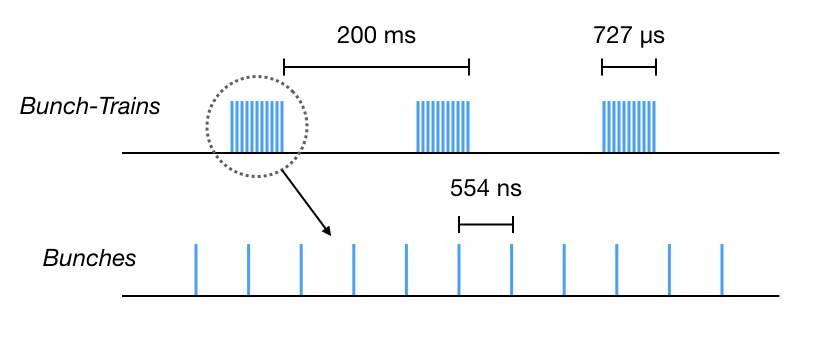
\includegraphics[width=0.7\linewidth]{chap2/fig/BeamStructure.jpeg}
  \caption{Schematic of beam structure of the ILC operated a design parameters.} \label{fig:ILC_BeamStruct}
\end{figure}


The electron beam is then transported by the Ring to Main Linac (RTML), accelerating electrons from 5 GeV to 15 GeV while compressing the bunch-length to few micrometers for the interaction region (IR).

The main linac of the ILC accelerates the electron beam up to 250 GeV by using superconducting RF cavities of niobium as shown in figure \ref{fig:CavityNiobium}. The cavities are operated at 2 Kelvins housed in cryomodules. The RF power is delivered by a system of Klystrons. The average gradient of the cavities is around 31.5 $\frac{MV}{m}$ with a quality factor $Q_0 \geqslant 10^{10}$. A demonstration of the mass-production and the operation of cryomodules which represents around 1\% of the ILC has been achieved for the synchrotron sources of FLASH and recently the European X-Ray Free Electron Laser (XFEL) \cite{Altarelli:2006zza} based at DESY.

\begin{figure}[htbp!]
  \centering
  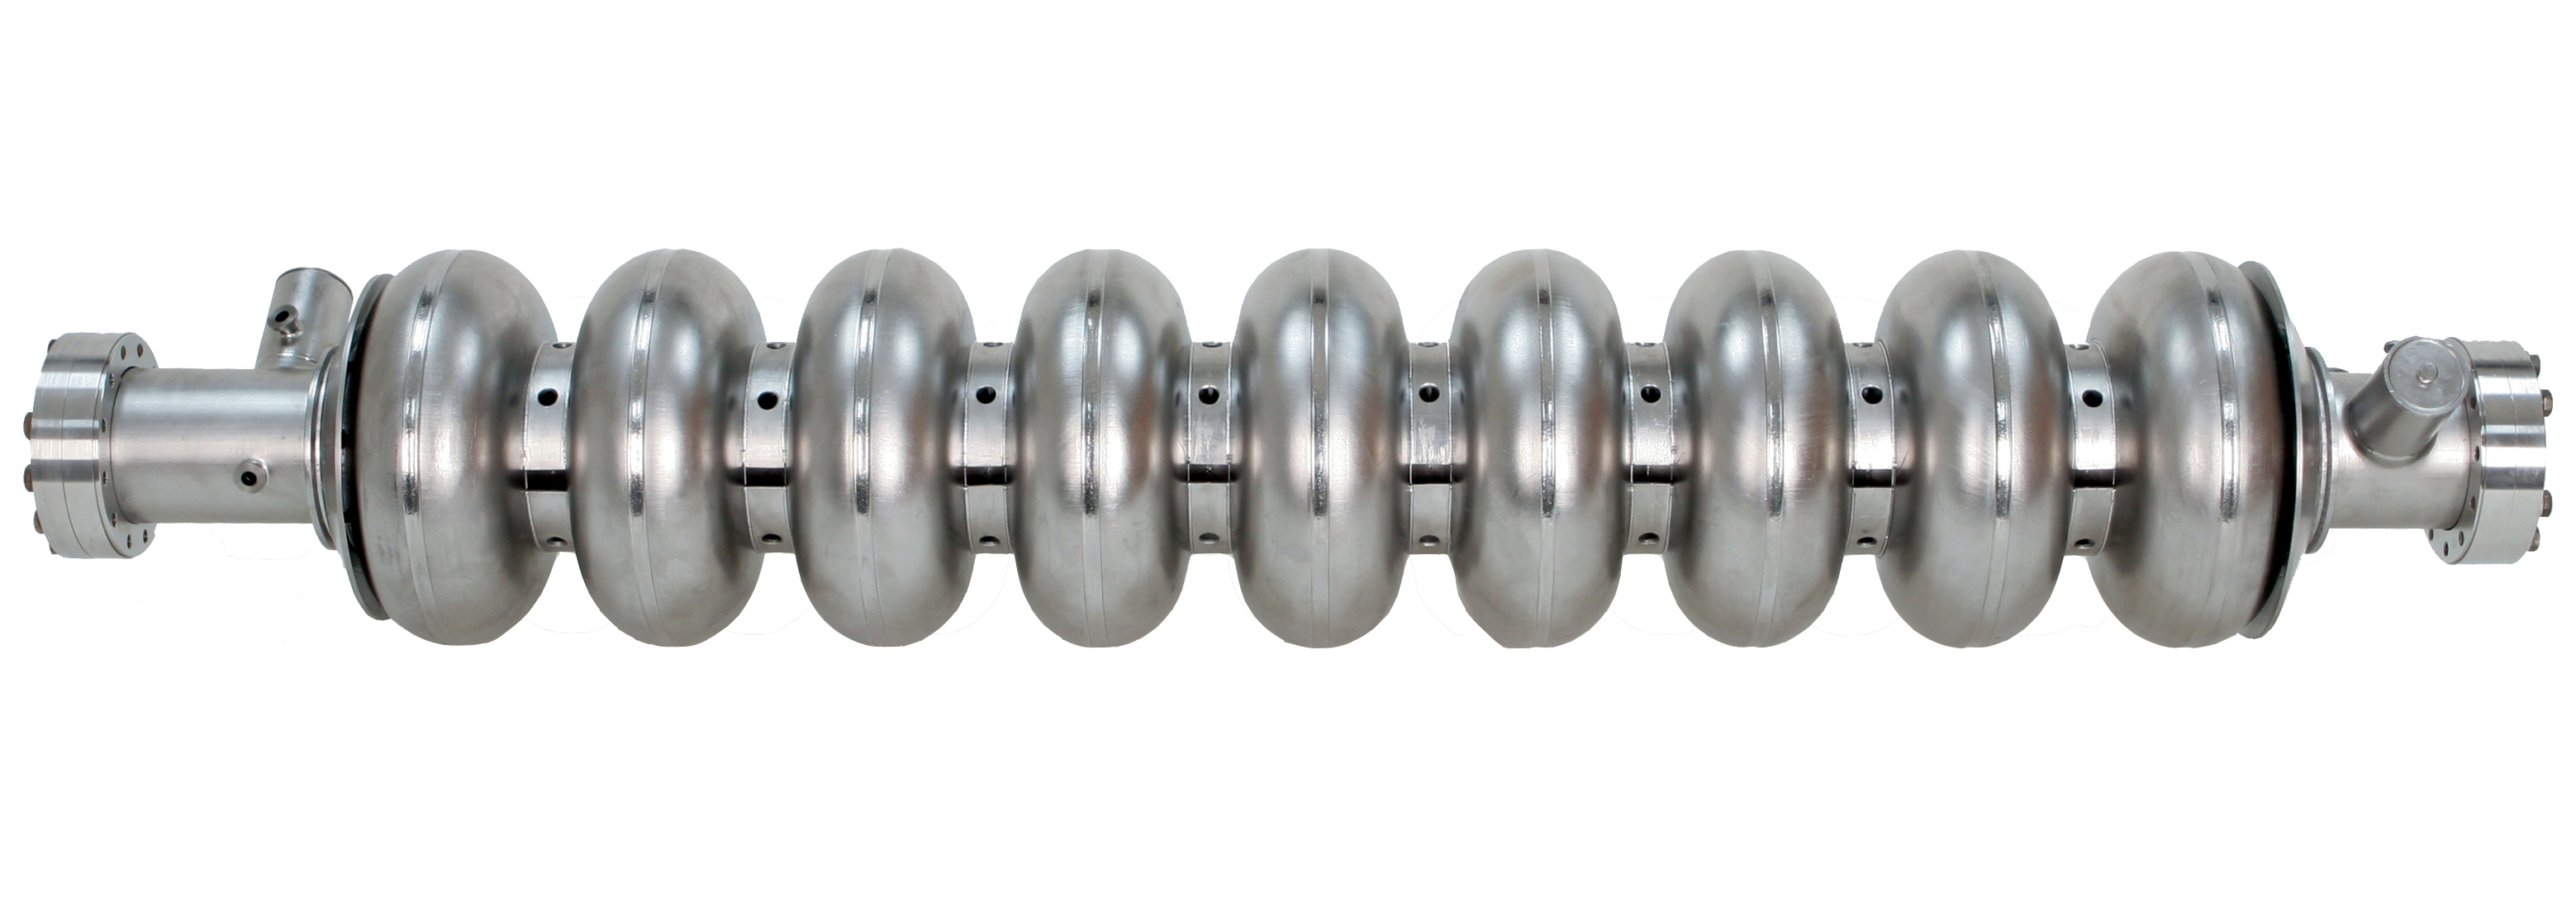
\includegraphics[width=0.7\linewidth]{chap2/fig/CavityNiobium.png}
  \caption{Picture of a nine-cell 1.3 GHz superconducting RF niobium cavity developed for the ILC. \cite{ILC_TDR_Vol3.1}.} \label{fig:CavityNiobium}
\end{figure}

After the acceleration, the electron beam is transported through a superconducting helical undulator which generates photons from 10 to 30 MeV. Then the electron beam is separated from the photon beam and transported by the Beam Delivery System (\acrshort{bds}) to the IR. The BDS is a complex system of different magnets and collimators which focuses the beam down to 474 nm $\times$ 5.9 nm (x and y respectively at $\sqrt{s} = 500$ GeV) to reach the luminosity goal of $2 \times 10^{34} cm^{-2}s^{-1}$.

The photons produced from the electron beam are directed onto a thin ($0.4 X_0$) titanium alloy (Ti) target producing elec\-tron\--positron pairs. The positrons are accelerated to 400 MeV in a first step while the remaining electrons and photons are dumped. Then, in a second step, they are accelerated to 5 GeV by a booster and injected into a damping ring, parallel to the electron ring. From there, the positron beam follows a second beam line that is similar to the electron beam line design and both beams are brought into collision at the IR, where the ILC detectors lie.

\subsection{Detectors}

The extensive ILC physics program (see section \ref{sec:ILC_Physics}) drives the requirements on the ILC detectors. In order to realize it, significant advances in detector performance are essential and many technological challenges must be overcome.

At the ILC, many physics processes have a hadronic jet final state. The requirement on the relative jet energy resolution at the ILC is driven by the separation of W and Z di-jet final states which is around 3-4\%. The current state of the art detectors cannot fulfill this requirement. The \textit{Particle Flow} approach (see section \ref{sec:PFA}) is an alternative method to traditional calorimetry that allows for better jet energy resolution. The Particle flow reconstruction requires a highly efficient tracking system and highly granular calorimeters.

At the ILC, two general purpose detector experiments are sharing the interaction region in a push-pull configuration. One detector occupies the IR while the other detector is parked in the detector hall. Both detectors can be moved in and out of the IR periodically every few weeks.

The requirements imposed by the physics program to the ILC detectors are \cite{ILC_TDR_Vol4}:
\begin{itemize}
  \item A relative jet energy resolution $\sigma_{E}/E$ between 3\% to 4\% for 100 GeV jets.
  \item A track momentum resolution $\sigma_{p}/p^2$ below $5 \times 10^{-5}$ GeV$^{-1}$.
  \item An impact parameter resolution below \SI{5}{\micro\meter} $\oplus$ \SI{10}{\micro\meter}/p(GeV/c) $sin^{3/2}(\theta)$ for an excellent flavor tagging (efficiency above 60\% for b jets).
  \item A low angle coverage for hermiticity.
\end{itemize}

The two detector concepts being developed for the ILC, the \textit{Silicon Detector} (\acrshort{sid}) and the \textit{International Large Detector} (\acrshort{ild}), are designed to fulfill the above requirements. In the following section, the ILD and SiD detector concepts will be briefly described.

\section{The International Large Detector (ILD)}
\label{sec:ILD}

The ILD detector is a multi-purpose detector. The tracking system and the calorimeter systems are both located within a superconducting solenoid magnet of 3.4 m radius providing a field of 3.5 T parallel to the beam axis. A schematic of the ILD detector is shown in figure \ref{fig:ILD}.

\begin{figure}[htbp!]
  \centering
  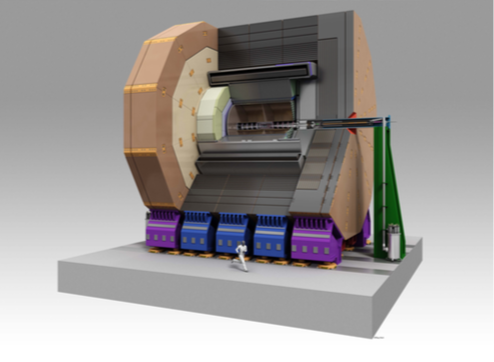
\includegraphics[width=0.6\linewidth]{chap2/fig/ILD_full.png}
  \caption{Schematic view of the International Large Detector. \cite{ILC_TDR_Vol4}} \label{fig:ILD}
\end{figure}

\subsection{The ILD Coordinate System}

The ILD coordinate system \cite{ILDCoordinates} is a right-handed Cartesian system with its origin at the nominal ILC interaction point. The z-axis is along the beam direction such as the z-component of the electron beam momentum is positive $p^-_z > 0$. The y-axis is pointing upwards. The x-axis then completes the Cartesian right-handed system.

\subsection{The ILD Tracking System}

The ILD tracking system is composed of multiple sub-detectors. A vertex detector (\acrshort{vtx}) is located near the beam pipe surrounded by the main tracker, a Time Projection Chamber (\acrshort{tpc}). Additionally, this is supplemented by few layers of silicon tracker between the VTX and the TPC (SET/SIT) and between the TPC and the calorimeters (ETD). Each subsystem is briefly described in the following.

\subsubsection{Vertex detector (VTX) and Silicon tracking system (FTD/SET/SIT/ETD)}

The vertex detector needs to fulfill the requirements of the ILC physics program by delivering an excellent flavor tagging performance of heavy quarks.

The ILD Tracking system consists of a multi-layer pixel vertex detector at the innermost part, at around 1.6 cm of the beam pipe. Different VTX geometries are proposed, a three double layer or a five single layer silicon pixel geometry. Additionally, two layers of silicon strip detector (\acrshort{sit}) are placed around the vertex detector to fill the gap between the VTX and the \textit{Time Projection Chamber} as well as two other layers of silicon strip detector (\acrshort{set}) are installed between the TPC and the calorimeters.

In the forward region, silicon pixel disks and silicon strip disks (\acrshort{ftd}) are installed to allow for tracking at low angles. Between the TPC endplate and the calorimeter endcaps, two silicon strip layers (\acrshort{etd}) are installed to improve tracking performance and to provide redundancy between the main tracking volume and the calorimeters.

The VTX offers position hit resolutions of less than \SI{6}{\micro\meter} \cite{ILC_TDR_Vol4} with a very low material budget of 0.15\% $X_0$ per layer. The SIT and FTD pixel detectors offer similar position hit resolutions with a material budget of 0.65\% $X_0$.

While the technology has not been decided yet for the VTX, several technologies are studied: CMOS Pixel Sensors (\acrshort{cps}) \cite{Winter:2012ms}, Fine Pixel CCDs (\acrshort{fpccd}) \cite{Murai:2016taa} and Depleted Field Effect Transistors (\acrshort{depfet}) \cite{Boronat:2016cog}. These technologies have the potential to fulfill the requirements of the ILD VTX.

\subsubsection{Time Projection Chamber (TPC)}

The main feature of the ILD tracking system is a large TPC that can provide more than 200 points per track, covering from 330 mm to 1808 mm in radius. The TPC consists of a gas sensitive volume that serves as detection medium. When a charged particle goes through the TPC, it ionizes the gas along its path. The free electrons produced via ionization drift towards the endplates of the TPC by applying an electric field parallel to the beam axis. The endplate detects the drifting electrons using a \textit{Gas Electron Multiplier} (\acrshort{gem}) \cite{Sauli:1997qp} or a \textit{Micro-Mesh Gaseous Structure} (\acrshort{micromegas}) \cite{Giomataris:1995fq} readout system. These technologies provide the amplification of the drifting electrons and give a two-dimensional position information.

The spatial resolution of the TPC is better than \SI{100}{\micro\meter} \cite{Mueller:301339} and also offer a double hit resolution in the order of less than 2 mm in $r\phi$. This resolution is worse than what silicon tracking can offer but the TPC presents the advantage of a very low material budget, continuous tracking and excellent reconstruction of the non-pointing tracks from multiple scattering. In addition, the TPC offers the possibility of particle identification via the specific energy loss measurement $\frac{dE}{dx}$ (see subsection \ref{sec:PartInter}) with a resolution of around 5\%.

A combined momentum resolution $\sigma_{p_T}/p_T^2$ of $2 \times 10^{-5}$ GeV$^{-1}$ has been achieved for high momenta for the ILD tracking system.

\subsection{The ILD Calorimeter System}

The ILD calorimeter system is designed and optimized for \textit{Particle Flow} (see section \ref{sec:PFA}). It is aiming to achieve a jet energy resolution $\sigma_E/E$ of around 3-4 \% in the energy range of 45 to 250 GeV. To achieve such goals, an unprecedented 3D granularity for the calorimeters is required combined with an excellent tracking reconstruction. To minimize material budget and optimize track associations to depositions in the calorimeters, the calorimeters are placed inside the solenoid magnet thus limiting the depth of the calorimeters. The ILD calorimeter system consists of an electromagnetic calorimeter (\acrshort{ecal}) and a hadronic calorimeter (\acrshort{hcal}).

The electromagnetic calorimeter needs to have an unprecedented granularity to fulfill the Particle Flow requirements. It needs to be able to separate showers created by different photons. Additionally, it plays an important role in hadronic shower start identification and separation as a significant fraction of hadron showers start in the ECAL. The baseline ECAL has 30 active layers using silicon-bas\-ed readout with a $5 \times 5$ mm segmentation in a tungsten absorber, allowing a very compact design. The total depth of the ECAL is of 24 radiation length. While the baseline uses silicon, a plastic scintillator strips technology is considered as an option. The two technologies can also be combined to reduce the overall cost of the detector while maintaining the performance.

The hadronic calorimeter measures the energy of hadrons. Following the particle flow approach, only the energy from neutral hadrons is measured in the HCAL, the energy of charged hadrons is measured in the tracker. Therefore, the HCAL needs to provide the necessary topological resolution power to separate charged and neutral hadron showers. The baseline HCAL has 48 active layers in a steel absorber of a depth of 6 nuclear interaction length. Two options are considered for the active layers: scintillator-tile based and gas-based technologies.

In the forward region, additional calorimeters are placed: LumiCal, BeamCal and LHCAL for luminosity monitoring, beamsstralhung measurement and hermiticity at low angles down to 5 mrad.

After the solenoid magnet, an iron yoke returns the magnetic field and is planned to be instrumented with scintillator strips or resistive plate chambers (\acrshort{rpc}) to serve as a muon detector and tail catcher for high energy jets.

\section{The SiD Detector}

The SiD detector concept is very similar to the ILD detector. It differs by its size much smaller than ILD, the use of a stronger magnetic field (5 T) and a full silicon tracking system instead of a TPC. The ECAL is also using silicon as active material. Resistive plate chambers (RPCs) with gas as active material were planned to be used for the hadron calorimeter system but a recent change in the baseline design includes now a scintillator-tile hadronic calorimeter. The performance of SiD is very close in numbers to ILD. A representation of the SiD detector is shown in figure \ref{fig:SiD}.

\begin{figure}[htbp!]
  \centering
  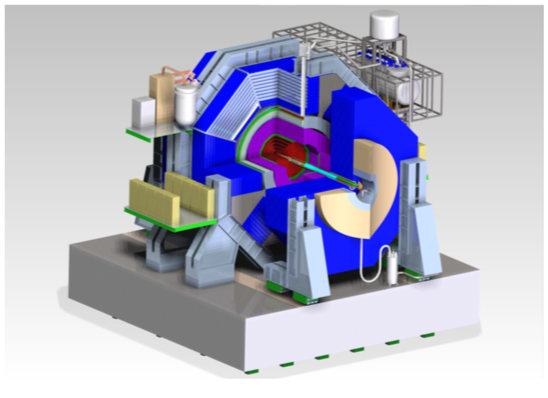
\includegraphics[width=0.6\linewidth]{chap2/fig/SiD_Detector.png}
  \caption{Schematic view of the Silicon Detector. The different sub-detector are shown: tracking (red), ECAL (green), HCAL (violet) and flux return yoke (blue).\cite{ILC_TDR_Vol4}} \label{fig:SiD}
\end{figure}

\section{The Compact Linear Collider (CLIC)}

Another concept that was aforementioned is the Compact Linear Collider (CLIC) \cite{Aicheler:2012bya, CLIC_CDR}. CLIC is drastically different than the ILC in the design and technology used. CLIC uses normal conducting copper cavities operated at 12 GHz which is much higher than ILC (1.3 GHz). The cavities have a much higher accelerating gradient at around 100 $\frac{MV}{m}$. Therefore, a center-of-mass energy up to $\sqrt{s} = 3$ TeV can be achieved while keeping the accelerator compact.

It uses a two-beam operation scheme where a drive beam provides the RF power to accelerate another beam. The beam structure is composed of bunch-trains separated by 20 ms. Each bunch-train consists of 312 bunch-crossings that are separated by 0.5 ns.

The CLIC detectors must meet at minimum the requirements of the ILC detectors. However, they must meet the requirements up to 3 TeV. Therefore, a higher magnetic field of 4 T and a thicker hadron calorimeter (50 active layers corresponding to 7.5 interaction length) using Tungsten as absorbing material is used. In addition, the detectors must be able to operate in the CLIC environment, e.g 0.5 ns bunch spacing, $\gamma\gamma \rightarrow$ hadrons background. Hence, an excellent time resolution for all detector components is needed.

The CLIC accelerator technology is yet not mature compared to the ILC and still needs several years of R\&D before a full CLIC accelerator could be constructed.

\begin{figure}[htbp!]
  \centering
  \begin{subfigure}{0.55\textwidth}
    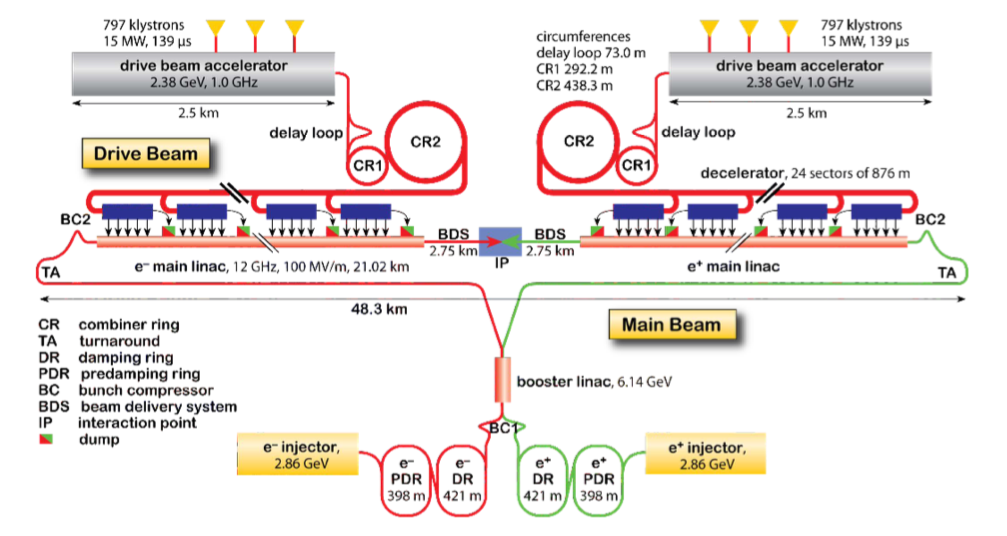
\includegraphics[width=1\linewidth]{chap2/fig/CLIC_Machine.png}
    \caption{} \label{fig:CLICMachine}
  \end{subfigure}
  \hfill
  \begin{subfigure}{0.44\textwidth}
    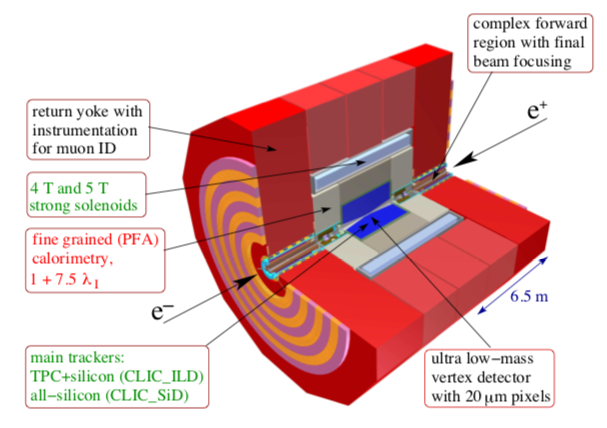
\includegraphics[width=1\linewidth]{chap2/fig/CLIC_DetConcept.png}
    \caption{} \label{fig:CLICDet}
  \end{subfigure}
  \caption{\subref{fig:CLICMachine}) Schematic view of the CLIC accelerator at $\sqrt{s}$ = 3 TeV \cite{Aicheler:2012bya}. \subref{fig:CLICDet}) Schematic overview of the CLIC detector concepts \cite{CLIC:2016zwp}.} \label{fig:CLIC}
\end{figure}

\begin{center}
  \rule{0.5\textwidth}{.4pt}
\end{center}

As discussed in this chapter, the ILC provides a clean environment combined with advanced detectors that allow for precision physics studies. To fulfill the ILC program, calorimeters are an essential tool in jet energy measurement and are designed for the Particle Flow approach. The concept of calorimetry and the Particle Flow paradigm are discussed in the next chapter.
